% Chapitre 4 : La Démarche

\section{Chapitre 4 : La Démarche}



La démarche de conception d'un logiciel définit la méthodologie suivie pour passer du besoin exprimé au logiciel opérationnel. Ce chapitre présente les méthodes de développement appliquées au projet SaaS Directory, en mettant l'accent sur l'approche orientée objet avec UML et en justifiant le non-recours aux méthodes formelles.



\subsection{Méthodes de Développement Semi-Formelles}



Le cours de Génie Logiciel présente plusieurs méthodes semi-formelles : SADT (Structure Analysis and Design Technique), MERISE (méthode française systémique avec séparation données/traitements), UML/Processus Unifié (itérative, incrémentale, orientée objet avec approches ascendante et descendante), OMT (Object Modelling Technique de James Rumbaugh), et OOSE (Object-Oriented Software Engineering d'Ivar Jacobson basée sur cinq modèles : besoins, analyse, conception, implémentation, test).



Pour SaaS Directory, nous avons retenu l'approche UML/Processus Unifié pour plusieurs raisons. Premièrement, son caractère itératif et incrémental correspond parfaitement à notre modèle de cycle de vie. Deuxièmement, son orientation objet s'aligne avec notre stack technologique (React composants, Drizzle ORM entités). Troisièmement, UML est devenu le standard industriel de facto pour la modélisation orientée objet, garantissant la lisibilité et la communication de nos modèles.



\subsection{Diagrammes UML Appliqués au Projet}



L'application d'UML à SaaS Directory se manifeste à travers plusieurs diagrammes standards, conformes aux spécifications OMG.



\subsubsection{Diagramme de Cas d'Utilisation}



Le diagramme de cas d'utilisation modélise les interactions entre les acteurs et le système. Les acteurs principaux sont : Visiteur, Utilisateur Authentifié, Créateur de Produit, et Administrateur. Les cas principaux incluent : s'authentifier, créer un profil, lancer un produit, voter pour un produit, commenter, envoyer un message, gérer son abonnement, et modérer le contenu.



\begin{figure}[H]

\centering

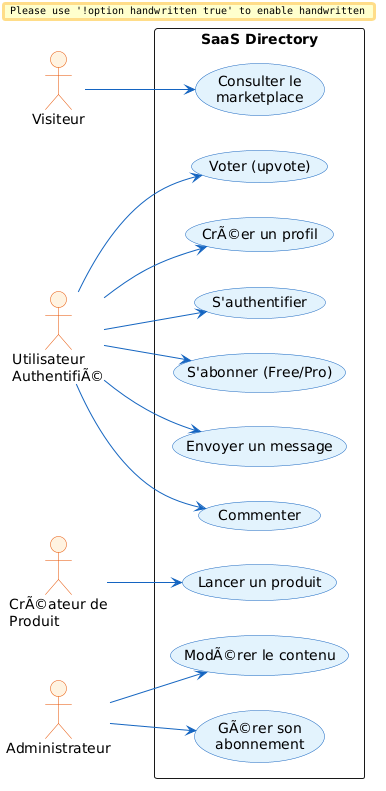
\includegraphics[width=0.95\textwidth]{assets/use_case.png}

\caption{Diagramme de Cas d'Utilisation — SaaS Directory}

\label{fig:use-case}

\end{figure}



La figure~\ref{fig:use-case} illustre les relations entre les quatre acteurs principaux et les cas d'utilisation du système. Le visiteur non authentifié peut consulter le marketplace. Une fois authentifié, l'utilisateur accède à l'ensemble des fonctionnalités sociales (votes, commentaires, messages). Le créateur de produit bénéficie de capacités de publication. L'administrateur dispose de privilèges de modération.



\subsubsection{Diagramme de Classes}



Le schéma Drizzle ORM dans \texttt{src/lib/db/schema.ts} constitue l'implémentation directe du diagramme de classes. Le système compte 20 tables regroupées en trois catégories.



\begin{figure}[H]

\centering

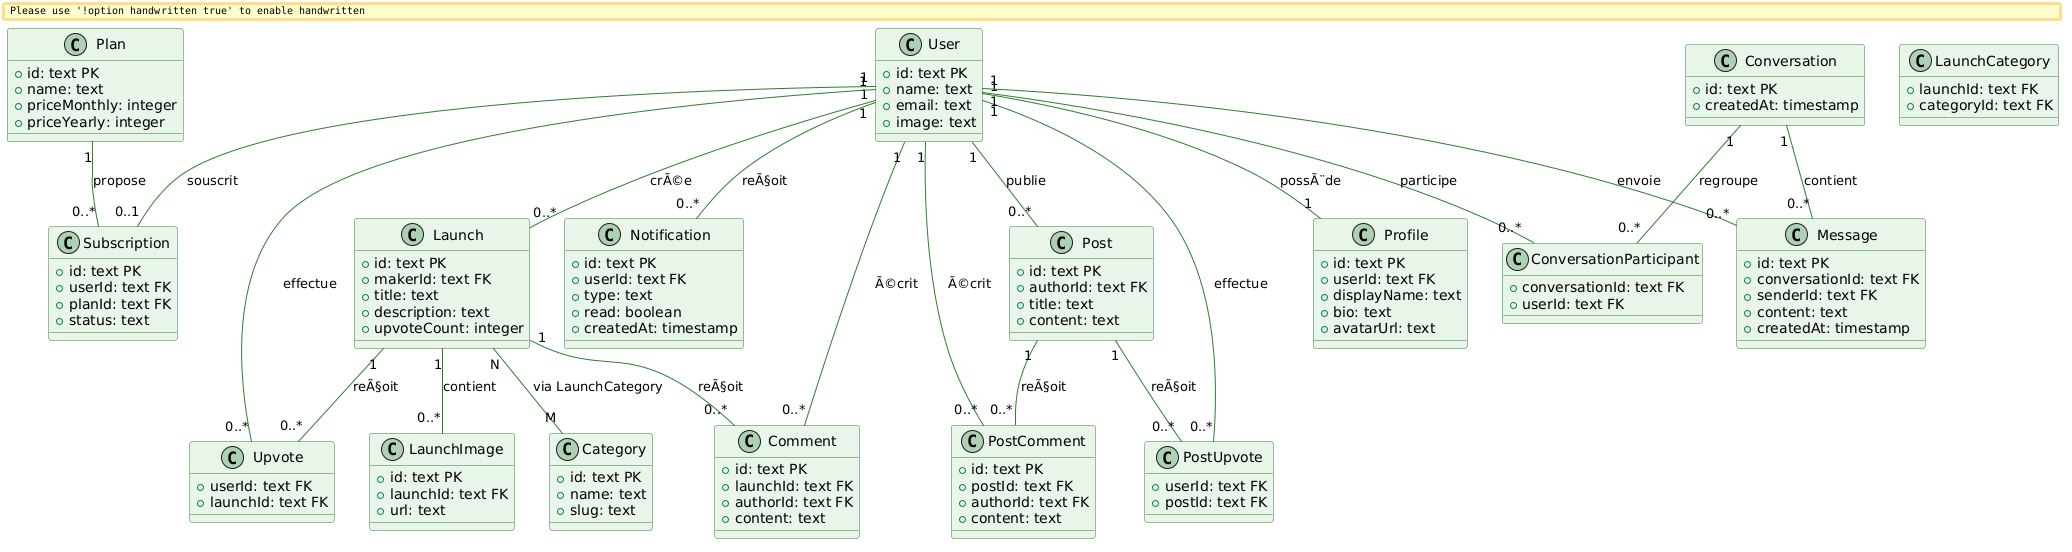
\includegraphics[width=0.95\textwidth]{assets/class.png}

\caption{Diagramme de Classes — SaaS Directory (20 tables)}

\label{fig:class}

\end{figure}



La figure~\ref{fig:class} présente l'architecture des classes avec leurs attributs et relations. Les \textbf{tables Better Auth} (\texttt{user}, \texttt{session}, \texttt{account}, \texttt{verification}) gèrent l'authentification. Les \textbf{tables métier principales} (\texttt{profile}, \texttt{launch}, \texttt{category}, \texttt{plan}, \texttt{subscription}) modélisent le cÅ“ur du marketplace. Les \textbf{tables d'interaction sociale} (\texttt{upvote}, \texttt{comment}, \texttt{post}, \texttt{postUpvote}, \texttt{postComment}, \texttt{conversation}, \texttt{conversationParticipant}, \texttt{message}, \texttt{notification}) gèrent la dynamique communautaire.



Les relations entre ces entités suivent le modèle relationnel classique : \texttt{User} possède un \texttt{Profile} (1:1), \texttt{User} crée des \texttt{Launches} (1:N), \texttt{Launch} appartient à des \texttt{Categories} (N:M via \texttt{launchCategory}), \texttt{User} reçoit des \texttt{Notifications} (1:N), et \texttt{User} participe à des \texttt{Conversations} (N:M via \texttt{conversationParticipant}).



\subsubsection{Diagramme de Séquence}



Le diagramme de séquence de la messagerie temps réel illustre l'interaction entre les acteurs et le système.



\begin{figure}[H]

\centering

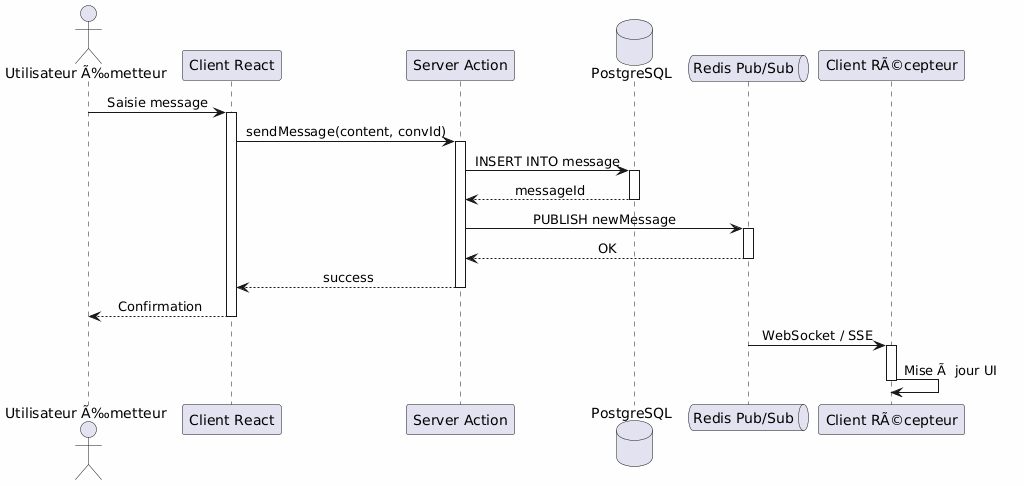
\includegraphics[width=0.95\textwidth]{assets/sequence.png}

\caption{Diagramme de Séquence — Envoi d'un Message en Temps Réel}

\label{fig:sequence}

\end{figure}



La figure~\ref{fig:sequence} montre le flux complet d'un message : l'utilisateur émetteur saisit le message via l'interface React. Le Client Component appelle la Server Action \texttt{sendMessage} qui insère le message dans la table \texttt{message} via Drizzle ORM. La Server Action publie ensuite un événement sur Redis Pub/Sub. Le serveur Redis notifie tous les clients abonnés à la conversation. Le Client Component récepteur reçoit la notification via WebSocket/SSE et met à jour l'interface sans rechargement de page. Ce flux démontre la séparation des préoccupations entre présentation, métier et persistance.



\subsection{Méthodes Formelles et Langage Z}



Les méthodes formelles (langage Z, B, VDM) utilisent des notations mathématiques pour spécifier, développer et vérifier des systèmes logiciels. Elles garantissent la correction du logiciel, éliminent les erreurs et facilitent la maintenance. Le langage Z, développé à l'Université d'Oxford par Jean-Raymond Abrial, est un langage de spécification formelle basé sur la théorie des ensembles, la logique des prédicats et un langage schématique pour structurer les spécifications.



Bien que puissantes, les méthodes formelles n'ont pas été utilisées dans ce projet pour plusieurs raisons pragmatiques. Premièrement, le domaine du marketplace web n'est pas critique au sens des systèmes embarqués ou médicaux où les méthodes formelles sont indispensables. Deuxièmement, la courbe d'apprentissage du langage Z est élevée et incompatible avec les contraintes temporelles d'un projet académique. Troisièmement, TypeScript et Zod fournissent un niveau de vérification formelle suffisant pour notre contexte (typage statique, validation de schémas à la compilation et à l'exécution).



Néanmoins, la compréhension des méthodes formelles reste essentielle pour apprécier les limites des approches semi-formelles et identifier les contextes où elles deviennent nécessaires.

